
%(BEGIN_QUESTION)
% Copyright 2006, Tony R. Kuphaldt, released under the Creative Commons Attribution License (v 1.0)
% This means you may do almost anything with this work of mine, so long as you give me proper credit

Suppose two water pipes of different diameter both have blunt objects (``bluff bodies'') in the paths of their respective water flows.  A pressure sensor device located near each of the bluff bodies measures the frequency of the vortices produced:

$$\includegraphics[width=15.5cm]{i00495x01.eps}$$

If the bluff bodies in both pipes have the same physical dimensions, and the vortex shedding frequencies are the same in both scenarios, which pipe carries a greater volumetric flow rate of water?  Or, do they carry the same amount of flow?  Why or why not??

\underbar{file i00495}
%(END_QUESTION)





%(BEGIN_ANSWER)

The large pipe carries a greater volumetric rate of water flow than the small pipe.

\vskip 10pt

Since the vortex shedding frequency is proportional to the fluid {\it velocity}, we know that the flow velocities in both cases must be the same (given identical bluff body geometries).  However, since the larger pipe has a greater cross-sectional area, an identical velocity equates to a greater {\it volume} rate of water moving past the bluff body and sensor.

%(END_ANSWER)





%(BEGIN_NOTES)


%INDEX% Measurement, flow: vortex shedding

%(END_NOTES)


